% This must be in the first 5 lines to tell arXiv to use pdfLaTeX, which is strongly recommended.
\pdfoutput=1
% In particular, the hyperref package requires pdfLaTeX in order to break URLs across lines.

\documentclass[11pt]{article}

% Remove the "review" option to generate the final version.
\usepackage[review]{ACL2023}

% Standard package includes
\usepackage{times}
\usepackage{latexsym}

% For proper rendering and hyphenation of words containing Latin characters (including in bib files)
\usepackage[T1]{fontenc}
% For Vietnamese characters
% \usepackage[T5]{fontenc}
% See https://www.latex-project.org/help/documentation/encguide.pdf for other character sets

% This assumes your files are encoded as UTF8
\usepackage[utf8]{inputenc}

% This is not strictly necessary, and may be commented out.
% However, it will improve the layout of the manuscript,
% and will typically save some space.
\usepackage{microtype}

% This is also not strictly necessary, and may be commented out.
% However, it will improve the aesthetics of text in
% the typewriter font.
\usepackage{inconsolata}
\usepackage{tabularx}
\usepackage{float}
\usepackage{listings}
\usepackage{pgfgantt}
\usepackage{amsmath}
\usepackage{longtable}
\usepackage[
backend=biber,
style=numeric-comp,
]{biblatex}
\addbibresource{bibliography.bib}

% If the title and author information does not fit in the area allocated, uncomment the following
%
%\setlength\titlebox{<dim>}
%
% and set <dim> to something 5cm or larger.

\title{Systematic literature review on open-source data warehouse tools and design trends}

% Author information can be set in various styles:
% For several authors from the same institution:
% \author{Author 1 \and ... \and Author n \\
%         Address line \\ ... \\ Address line}
% if the names do not fit well on one line use
%         Author 1 \\ {\bf Author 2} \\ ... \\ {\bf Author n} \\
% For authors from different institutions:
% \author{Author 1 \\ Address line \\  ... \\ Address line
%         \And  ... \And
%         Author n \\ Address line \\ ... \\ Address line}
% To start a separate ``row'' of authors use \AND, as in
% \author{Author 1 \\ Address line \\  ... \\ Address line
%         \AND
%         Author 2 \\ Address line \\ ... \\ Address line \And
%         Author 3 \\ Address line \\ ... \\ Address line}

\author{Jurgen Grotentraast \\
  Student Data Science \& technology\\
  University of Twente \\
  j.grotentraast@student.utwente.nl\\}

\begin{document}
{\makeatletter\acl@finalcopytrue
  \maketitle
}
\begin{abstract}
As data is still becoming a bigger asset every day, data warehousing is a very common practice for businesses to show trends, averages, and bottlenecks in processes. To create such a data warehouse, a plethora of tools are available and even more design methodologies have been proposed over the years. Current research has not given a clear overview of available open-source tools that can be used to create a data warehouse.  On the other hand, research available on design and implementation trends for data warehouses only reflects everything before 2017. Therefore, the contribution of this paper is twofold. First, an overview of available open-source data warehouse tools was created based on literature and search engine results. To ensure these tools are a viable, future-proof option they should be last updated in or after 2023. Second, a systematic literature review was performed to find current trends or approaches for the research, design, development, implementation, or improvement of a data warehouse. This covers trends that have emerged since 2017 to see whether old trends are still being pursued or if new trends have emerged to continue where previous research on this topic has stopped. 
\end{abstract}

\section{Introduction}
With the still-growing value of data in today's world, many organizations have invested in the development of a data warehouse (DW). A data warehouse is used to store data differently to efficiently analyze business data \cite{gupta1997selection}. Data warehouses can be used for analyzing and improving business processes \cite{shahzad2009goal}, but also to get a better understanding of for example the financial situation of an organization \cite{lapura2018development}. A data warehouse utilizes historical data to show trends, averages, and bottlenecks in a process or production chain and to show what areas of this process or production chain can be improved \cite{Chaudhuri1997}. \\

A data warehouse captures data from one or multiple sources, transforms the data in such a way that aggregations on this data are easy and fast to execute, and finally loads this data into the data warehouse database. This process is called extract-transform-load (ETL). Over the years many tools and software solutions have been developed to aid people in this process. Some tools are purely programming libraries or extensions that help the user to achieve what they want \cite{Thomsen201821, Jensen202145, Biswas_programming2019267}, whereas other software applications are developed further such that they can be used to build ETL pipelines with minimal coding. Companies like Amazon, Microsoft, and Google have developed such software applications for creating data warehouse solutions. However, these are often very expensive and require a subscription to their entire cloud platform to use them. Fortunately, over the last couple of years, open-source data warehouse tools have been developed further and further \cite{nejres2015analysis}. This means that open-source tools now have the same functionality as expensive enterprise solutions. Furthermore, these open-source tools allow the user to build upon the tool themselves if something is missing. For example, if a connection to a specific source of data is not yet part of the tool, the user can build a custom connector through for example an API and still extract all the data they want. \\

Designing a data warehouse can be done in various ways. Each approach has its advantages and disadvantages. The approach that works best for a company or person depends on various factors including the use-case of the data warehouse and the background of the designer. Over the years these approaches have been further evolved and new trends have emerged. As discussed in more detail further on, literature of the past years has extensively researched the trends of the approach of the design, development, implementation, and improvement of a data warehouse \cite{costa2018evaluating, kozmina2018information, golfarelli2017star, chandra2018comprehensive}. \\

\section{Problem statement}
With the large amount of open-source tools available and the continuously changing trends in the approach or methodology of the design, development, implementation, or improvement of data warehouses, a clear overview of currently available tools and current trends is missing. Literature up until now has shown trends that were emerging up until 2018/2019 \cite{costa2018evaluating, kozmina2018information, golfarelli2017star, chandra2018comprehensive}, but whether those trends are still relevant and what other trends have emerged since then is unknown at the time of writing. 

\subsection{Research questions}
Therefore, for this review, two main research questions were created. Answering these questions will give insight into current developments in open-source ETL tools as well as DW trends that have emerged over the past five years.

\begin{itemize}
    \item \textbf{RQ1}: What open-source tools were last updated in or after 2023 are currently available?
    \item \textbf{RQ2}: What are trends and approaches in the research, design, development, implementation, and improvement of a data warehouse from 2018 up until 2024?
\end{itemize}


\section{Methodology}
\label{methodology}
A literature review was conducted for both research questions, where the tools found for \textbf{RQ1} found in the literature were extended with tools found on the internet. The methodology is based on the guidelines of Kitchenham et al. \cite{kitchenham2015evidence}. Both literature studies had a population of published studies from 2018 up to and including February 2024. All papers are written in English and are published in the field of computer science. For both literature studies, Scopus was used as the library of choice as it was indicated as the most comprehensive and user-friendly literature database \cite{harzing2016google, mongeon2016journal}.\\

\subsection{Search strategy}
\label{searchstrat}
For both literature studies, a search query was created through a process of trial and error to see which combination of keywords and query composition returned the best results. Next, inclusion and exclusion criteria were created. For \textbf{RQ1}, criteria were created for both the research papers as well as for the tools. For \textbf{RQ2}, criteria were only created for the papers. \\

\subsubsection{Tools}
\label{searchstrat:tools}
To answer the first research question, a combination of results from literature and the internet was used. Since the goal of this research question is to find all available tools that are currently popular, using only literature was not an option as this would yield a very limited result and would not be a representative overview of the software that is available. The following search query was used for finding literature: \\

\textbf{(open-source OR "open source") AND ("data warehouse" OR etl) AND (solution OR tool)}\\

The search was done in the title, abstract, and keywords of the study. The result was a set of 65 papers. These papers, however, were not all relevant. Therefore several inclusion criteria (IC) for the papers were set up. As mentioned before, the goal is to find tooling which should be considered in the proposed research. Therefore, there are only two inclusion criteria.

\begin{itemize}
    \item \textbf{IC1}: The subject of the paper should be data warehousing or ETL.
    \item \textbf{IC2}: The paper should mention the tools that were used for the research.
\end{itemize}

The above-mentioned IC were applied while reading the title and abstract of each paper, this resulted in 18 papers being left. These 18 papers were carefully read to find any tool that was mentioned. This initial result was extended with tools found through a Google search. For this search the following queries were used:

\begin{itemize}
    \item open source data warehouse tools
    \item open source etl tools
\end{itemize}

The resulting pages included rankings of the so-called "best" ETL or data warehouse tool to forums discussing different possibilities for tools that can be used to develop and run ETL pipelines. The complete list of tools that were found can be seen in table \ref{table:tools}. However, not all of these tools should be taken into consideration for the proposed research. Therefore, new inclusion and exclusion criteria for the tools were formed.

\begin{itemize}
    \item \textbf{IC1}: The tool has to be open-source
    \item \textbf{IC2}: The source code should be accessible
    \item \textbf{IC3}: The latest release should be in or after 2023
    \item \textbf{EC1}: The tool is operating system specific
\end{itemize}

After applying the inclusion and exclusion criteria for tools to the initial list of tools there remained 25 tools. For a visual overview of this process see figure \ref{fig:tools}.

\begin{figure}
\centering
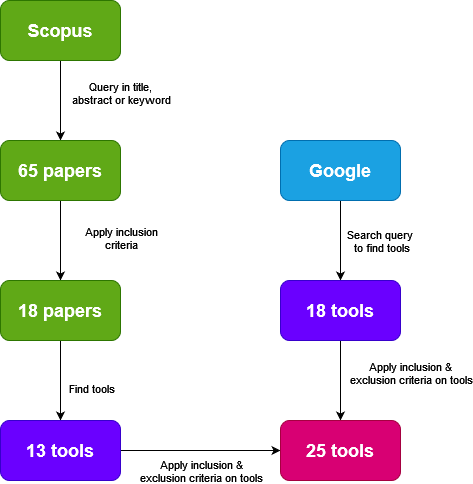
\includegraphics[scale=0.5]{Images/Tools.drawio.png}
\caption{Tool selection process}
\label{fig:tools}
\end{figure}

\subsubsection{Trends \& approaches}
\label{searchstrat:trends}
To answer the second research question, a second literature study was performed. The population was the same as for the first, except that this study was additionally limited to conference papers, articles, and book chapters. For this second part, the following search query was used:\\

\textbf{"data warehouse" AND  (design OR concept OR methodology)}\\

The search was again done in the title, abstract, and keywords of the study. The result was a set of 743 papers. These papers, however, were not all relevant. Therefore several inclusion criteria for the papers were set up. For this study, the quality of the papers did matter, as the goal of this part is to find current trends and problems found in research in the domain of, the design of, and the development of data warehouses. Therefore, the following inclusion criteria were formed:

\begin{itemize}
    \item \textbf{IC1}: The paper directly addresses a trend or problem with a solution or approach for the design, development, implementation, or improvement of a data warehouse
    \item \textbf{IC2}: The paper is peer-reviewed
    \item \textbf{IC3}: The paper is written in clear English
    \item \textbf{IC3}: The paper is available for download
\end{itemize}

An exclusion criterion was also formed to ensure the inclusion of only relevant information further.
\begin{itemize}
    \item \textbf{EC1}: The paper discusses the implementation of a data warehouse in a specific field without explicitly addressing and explaining a trend, problem, or approach in the design, development, implementation, or improvement of a data warehouse
\end{itemize}

After applying the above criteria while reading the title and abstract there were 231 papers left initially. Some papers were initially included but were rather ambiguous. These ambiguous cases were analyzed in further detail to ensure that all non-relevant papers were excluded, this further analysis resulted in 126 papers. These ambiguous cases included terms like "detailed description of design method" in the abstract, however, in the paper itself this only included what the star schema and ETL process looked like. Since this was not relevant to this literature study, these papers were still excluded. For a visual overview of this process see figure \ref{fig:trends}.\\

\begin{figure}
\centering
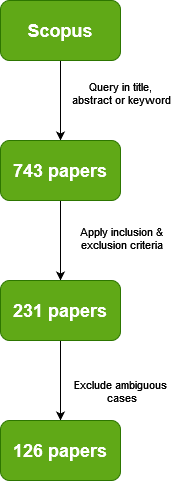
\includegraphics[scale=0.6]{Images/Trends.drawio.png}
\caption{Paper selection process}
\label{fig:trends}
\end{figure}

\section{Results \& Discussion}
\label{results}
The following sections show the tools that were identified in the literature and the ones that were found on Google as well as the trends and approaches that are currently of interest in research, design, and development regarding data warehouses. \\

\subsection{Tools}
\label{results:tools}
The final list of tools to answer \textbf{RQ1} consists of 25 tools. The first IC resulted in Talend, StreamSets, and Keboola being dropped. While Talend has been one of the biggest names in the open-source data warehouse industry, its software is no longer open-source as of 31st of January 2024. Keboola and StreamSets were also dropped because only a part of their tool was open-source but required the non-open-source part to work. \\

The second IC resulted in the exclusion of Hevo, as the source code for their platform was not accessible at all nor could the open-source license the software falls under be found. The third criterion was created to ensure that the software is still being kept up to date in terms of security and modern technologies. Therefore, Scriptella was excluded for example. Scriptella’s latest release was in October 2019 and no new release has been announced or planned since then. The software also uses rather outdated technology and is therefore not seen as a future-proof solution. \\

The exclusion criterion resulted in Open XDMoD being excluded. Open XDMoD is an ETL tool that can only run on Linux-based systems. This is not necessarily a bad thing, however, in this review, the tools should depend on areas like use cases and employee knowledge not on the operating system someone is running. \\

\begin{table*}
\centering
    \begin{tabular}{|c|c|}
        \hline
        \textbf{Tools found on web} & \textbf{Tools found in literature} \\ \hline
        Airbyte & Apache Druid \cite{Dymora202363} \\ \hline 
        Apache Airflow & Apache Hadoop \cite{Song2018233, Yoo2019476, Dymora202363} \\ \hline  
        Apache Beam & Apache Hive \cite{Yoo2019476, HouSu20221581, Dymora202363, Camacho-Rodríguez20191773} \\ \hline  
        Apache Camel & Apache Kafka \cite{Dymora202363} \\ \hline
        Apache Hop & Apache Spark \cite{Song2018233} \\ \hline  
        Apache NiFi & {\color[HTML]{FE0000} Hevo Data \cite{Sreemathy20211650}} \\ \hline  
        Apache SeaTunnel & {\color[HTML]{FE0000} OpenXDMoD \cite{Dean2022}}  \\ \hline  
        CloudQuery & Pentaho Community Edition \cite{Sreemathy20211650, Fang2022, Zheng2023} \\ \hline  
        Dagster & Python libraries\text{*} \cite{Fissore2018267} \\ \hline  
        DBT & R\_etl \cite{Biswas_programming2019267, Biswas_realtime202053} \\ \hline  
        {\color[HTML]{FE0000} Keboola} & {\color[HTML]{FE0000} Scriptella \cite{Biswas_programming2019267, Biswas_realtime202053}}\\ \hline
        Kestra & {\color[HTML]{FE0000} StreamSets \cite{Sreemathy20211650}} \\ \hline
        Knime Analytics Platform & {\color[HTML]{FE0000} Talend \cite{Espinoza2023, Sreemathy20211650}} \\ \hline
        Mage & \\ \hline
        Meltano & \\ \hline
        Prefect & \\ \hline
        PipelineWise & \\ \hline
        Singer & \\ \hline
    \end{tabular}
    \caption{The complete list of tools that were found before applying the criteria. The tools that were excluded after applying the criteria are marked in red. Tools on the right were found in literature, and tools on the left were found through the accommodating web search. \\
    \text{*}The Python libraries include: Ethereum-etl \cite{Camozzi2022},  Luigi, Petl \cite{Biswas_programming2019267, Biswas_realtime202053}, and Pygrametl\cite{Thomsen201821, Jensen202145, Biswas_programming2019267, Biswas_realtime202053}}
\label{table:tools}
\end{table*}

The tools that were no longer included after applying the inclusion and exclusion criteria are marked in red in table \ref{table:tools}. The left side shows the tools that were found on the internet. The right side shows tools that were found in the literature with the corresponding paper referenced. \\

The papers of Yu et al. and Spengler et al. \cite{Yu2022, Spengler2020415} are not mentioned in the table as these papers described the process of creating their own ETL tool from scratch. While the paper of Fissore et al. is mentioned in the table, it should be noted that this paper did not use any specific tool or library. Instead, they used basic Python functionalities to take care of their ETL process. However, since these have very specific purposes these are not taken into consideration. A more comprehensive overview of the included tools can be found in appendix \ref{appendix:tools}. This appendix shows some basic information about each tool including if the tool uses a specific programming language or is more low/no code; the size of the GitHub contributors and the number of stars the repository has; if the tool has a non-open-source paid option with more functionalities; and an optional small note for interesting capabilities, weaknesses or other noteworthy findings of the tool. This information was gathered through the website of each respective tool. \\ 

As mentioned in the methodology in section \ref{searchstrat:tools}, the results consist of tools found in literature and through a search engine. The reason for this is that most tools that are used daily are used by companies that are not involved in research. Furthermore, the tools themselves are not created for research purposes but instead are developed as business tools to aid businesses in gaining business intelligence and performing data analytics. Therefore, these tools can not be found in literature studies. To ensure this, tools that were found through the search engine were also queried through Google Scholar to see if the initial literature search might have missed papers in which these tools were mentioned. These extra searches did not yield any new results. 


\subsection{Trends in literature}
\label{results:trends}
The following sections will discuss the trends found in the literature regarding data warehouse design in more detail and therefore answer \textbf{RQ2}. The papers were divided into the following six categories:

\begin{enumerate}
    \item Data warehouse architecture
    \item Data warehouse design
    \item Data types
    \item ETL
    \item Performance
    \item Schema design
\end{enumerate}

Figure \ref{fig:papers} shows the distribution of the published papers over the years for each category. In each section one of the categories is further divided into trends regarding specific topics, these are presented in tabular form and explained in more detail afterwards.

\begin{figure*}
\centering
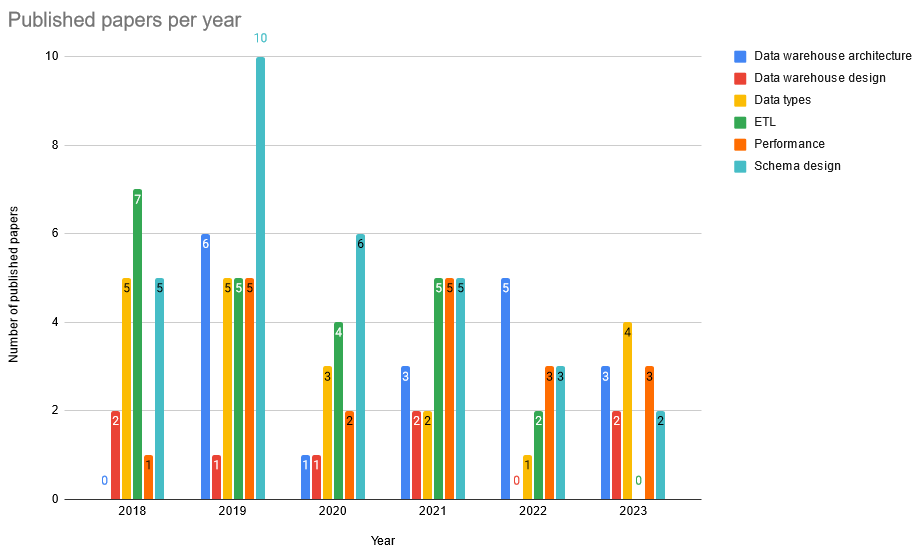
\includegraphics[scale=0.75]{Images/Papers per year2.0.png}
\caption{The number of papers published each year for every category}
\label{fig:papers}
\end{figure*}

\subsubsection{Data Warehouse architecture}
\label{results:trends:architecture}
The biggest trend that emerged in the literature on data warehouse architecture is the development of the Data Lake (DL). No papers were found that were published in 2018, but in 2019 several papers were published describing what a DL is; how it works; why it might be better than a traditional DW combined with limitations of traditional DWs; but also challenges that might need to be overcome to successfully use a DL \cite{Ravat2019304, Giebler2019179, Kachaoui2019}. This trend continued through to 2023 with the introduction of new design approaches; more DW limitations compared to the use of a DL; DL implementations with findings on challenges that were overcome; and finally in 2023 a paper describing the DL so far \cite{Liu2020, Chen2022405, Li2023, Singh2022530, Schering2022783, Oukhouya2023332}. These publications show a trend of high-level research on DL still focussed on what it is and what its benefits are. The challenges mentioned in the papers do change indicating that the DL is evolving and getting better although this is not specifically reflected in the topics discussed in the literature on DLs. A reason for this could be that this development takes place more on the commercial side rather than the research side and is therefore only reflected in research afterward.

Other topics that were mentioned in combination with DL throughout time were data quality and metadata systems. Both topics started emerging in 2019 \cite{Sawadogo2019440, Sawadogo2019558, Derakhshannia2019302}, but continued throughout time with new studies on data quality published in 2022 \cite{Azeroual20223} and studies on metadata published in 2021 \cite{Sawadogo202188}. Although not a definitive trend yet, it shows the divergence of high-level research previously discussed into more specific problems and areas that are now tackled within the literature. 

This divergence from high-level research is also seen in the other topics that were found. First is the emergence of the Lakehouse and the Data Mesh in 2021 \cite{Machado2021263, Orescanin20211242}. The Lakehouse was also studied in 2022 \cite{Behm20222326} by creating a faster query engine, indicating this topic might be going much faster than the DL itself, as improvements are already introduced rather than high-level conceptualizations, even though it stemmed from the DL. The data mesh was further studied in 2023 \cite{Vlasiuk2023183}, this study still focuses on the concept of a data mesh itself similar to the DL. See figure \ref{fig:arch} for a graphical overview. \\

\begin{figure*}
\centering
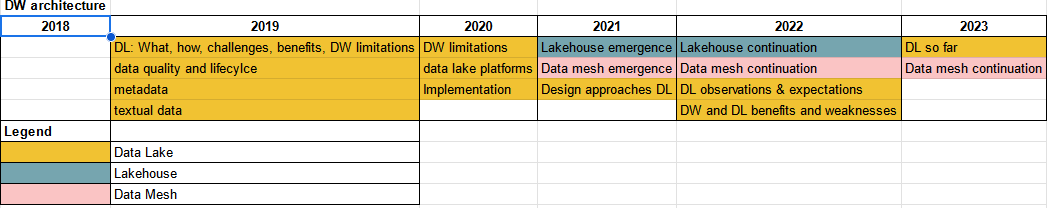
\includegraphics[scale=0.6]{Images/architecture.png}
\caption{Categorizations of trends for DW architecture}
\label{fig:arch}
\end{figure*}

\subsubsection{Data warehouse design}
\label{results:trends:design}
Even though the design method of Kimball was already introduced in 2002 \cite{kimball2011data}, throughout the studied years this design method was still being used as the basis for data warehouse design. While most papers simply describe and apply the method of Kimball \cite{Ramadhani202188, Himami2021146, Wahyudi2019, Rahutomo2018128}, some studies did build upon the existing methodology and improve it by introducing several hybrid approaches \cite{Takács20201}. This suggests that although already quite old, the methodology of Kimball is still proven useful and relevant. \\

In 2018, Uvidia et al also proposed a new version of another methodology for data warehouse design called HEFESTO 2.0 \cite{uvidia2017moving} however this did not catch on as no other papers on this topic were published between 2018 and 2024. Furthermore, no new design methods were developed during the studied years nor were other design methods covered or improved. \\

In 2023 there were two more papers published regarding the topic of data warehouse design. One covered the implications of Brewer's rule in data warehouse design \cite{raman2023implications} and the other discussed an approach and several guidelines for creating a sustainable green data warehouse \cite{letrache2018green}. Whether these topics become relevant trends in data warehouse design is yet to be seen as they were published near the end of the covered time period. \\

The one trend that was found only confirms that the method developed by Kimball et al. in 2002 remains relevant to this day. See figure \ref{fig:design} for a graphical overview. \\

\begin{figure*}
\centering
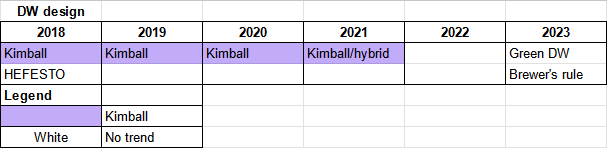
\includegraphics[scale=0.75]{Images/Design.png}
\caption{Categorizations of trends for DW design}
\label{fig:design}
\end{figure*}

\subsubsection{Data types}
\label{results:trends:types}
In 2018, a few trends arose regarding specific data types. First, two papers started researching ways to model trajectory data \cite{Azaiez2018353, Zekri2018380}. Second, studies began working on incorporating Linked Open Data (LOD) and semantic data into the ETL process \cite{Khouri2018, Khouri20181, Berkani20181}. In 2019 LOD continued to be a topic of interest \cite{khouri2019data}, while documented-oriented databases and NoSQL became a topic too either by itself \cite{Artamonov2019794, Bouaziz2019221} or in combination with geospatial data \cite{Ferro2019221}. Lastly, for 2019, interest was shown in Internet of Things (IoT) data \cite{Rahman2019181}. In 2020 LOD was still being researched \cite{Berkani2020397} and IoT data was also still being researched \cite{Plazas202084}. 2020 also showed the first sign of mixing two trends, with one paper studying the combination of trajectory and semantic data to see if trajectory data could be fit into a semantic data structure \cite{RodriguezBrisaboa2020113}. In 2021 the NoSQL data structure came around again with two more papers \cite{Bouaziz2021129, Banerjee2021162} and in 2022 Khalil et al. looked deeper into one type of NoSQL database, namely a graph-oriented one \cite{Khalil2022547}. \\

Several of the papers mentioned in the paragraph above that look into NoSQL \cite{Liu202334, Artamonov2019794, Bouaziz2019221, Bouaziz2021129, Banerjee2021162, Khalil2022547} are closely related to the Data Lake and Lakehouse architectures that were discussed in section \ref{results:trends:architecture}. These Data Lake and Lakehouse architectures are needed to store the NoSQL or document-oriented data that is discussed in this section. Furthermore, research into semantic data or LOD is also very popular as will also be seen in section \ref{results:trends:ETL} and section \ref{results:trends:schema}. The other trends on IoT and trajectory data were smaller but did show that specific data types or the nature of the gathered data does impact the ETL or Data Warehouse design. See figure \ref{fig:types} for a graphical overview. \\

\begin{figure*}
\centering
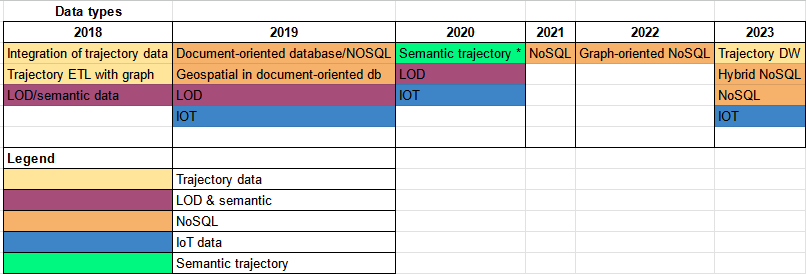
\includegraphics[scale=0.75]{Images/Types.png}
\caption{Categorizations of trends for Data types}
\label{fig:types}
\end{figure*}

\subsubsection{ETL}
\label{results:trends:ETL}
In 2018 three main trends emerged regarding ETL design. The first, while closely related and slightly overlapping with section \ref{results:trends:types}, is research on ETL design based on the type of data \cite{Mallek2018798, Teixeira2018225, Berkani201898}. The second trend is regarding ensuring or enhancing data quality within the ETL process \cite{Pan2018275}. The third trend is regarding real-time ETL, with one paper focussing on real-time ETL as a whole \cite{MohammedMuddasir2018436}, one paper focussing on using semantic data for real-time ETL \cite{Berkani20181}, thus combining the first and third trend, and one paper more specifically on utilizing Change Data Capture (CDC) to achieve real-time ETL \cite{Chandra2018}. \\

2019 mostly continued the second trend, with two more papers on assuring data quality \cite{Amuthabala2019233, Sreemathy20191183} and one paper on data enrichment using data mining \cite{Madhikerrni2019174}. Furthermore, two papers were published on expressing ETL processes using Business Process Modeling Notation (BPMN) to make ETL processes more interchangeable across tools \cite{Awiti2019299, Awiti2019427}. However, this topic did not become more relevant throughout the years. \\

In 2020 the second trend on data quality was again continued with one paper developing a framework for more general use to ensure a minimum level of data quality \cite{Ali2020}. Furthermore, the third trend on real-time ETL continues by mixing with the second trend on data quality with one paper. This paper studies the anomalies that arise when dealing with real-time ETL and how to overcome them \cite{MohammedMuddasir2020545}. Then a small trend emerges with ETL design based on metadata \cite{Wang2020}. Finally, there is one paper published on quality metrics for the entire ETL process \cite{Saebao2020539}, however, this does not evolve into an actual trend. \\

This small trend on metadata has one more paper in 2021 \cite{Panfilov2021139}, however, if this trend continues beyond 2021 is not entirely certain. No other papers on this topic were found in the population, but it might become more relevant in the future. Furthermore, in 2021 two more papers on ETL design based on data type were found. One on the impact of user-generated content on ETL design \cite{Walha2021374} and one on high-level ETL for semantic data warehouses \cite{DebNath202185}. Again there is a correlation between these papers and the papers covered in section \ref{results:trends:types}, but \cite{Walha2021374, DebNath202185} focus more on the ETL whereas the papers in \ref{results:trends:types} focus more on the entire Data Warehouse. Lastly, for 2021, there are two more papers on real-time ETL \cite{DeAssisVilela2021556, Ghosh2021585}. \\

In 2022 only the trend on the topic of data quality and enrichment remained with two more papers, one on data cleaning inside the ETL process \cite{Wrembel20223} and one on dynamic ETL for handling missing data \cite{BadiuzzamanBiplob2022243}. No papers were found on any of these topics in 2023. \\

Overall, these results mostly indicate the importance of data quality. Without clean data, a DW will not be of any help. The trends on types presented in this section and section \ref{results:trends:types} show that the type of data or data source will also greatly impact both the ETL process and the DW design. Lastly, many papers on real-time ETL were published showing the importance of the availability of the most up-to-date data. See figure \ref{fig:etl} for a graphical overview. \\

\begin{figure*}
\centering
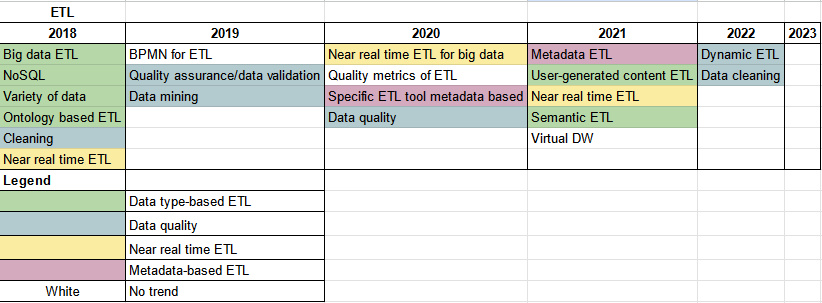
\includegraphics[scale=0.75]{Images/ETL.png}
\caption{Categorizations of trends for ETL}
\label{fig:etl}
\end{figure*}

\subsubsection{Performance improvement}
\label{results:trends:performance}
The biggest trend found regarding performance is regarding data placement and partitioning strategies. This trend started in 2018 with one paper \cite{Abbasi201863} with a strategy for predictable query times. In 2019 four more studies were published proposing new strategies to improve query time \cite{Du2019211, Ramdane2019189, Ramdane2019255, Kechar2019}. One more study was published on this topic in 2020 proposing the decoupling of data management and computation \cite{Liu202052}. In 2021 one study was published shifting the focus onto data placement strategies for Big data by dividing the data into themes \cite{Nie2021135} and one other study closely related to the topic of data placement which focused on materialized views to enhance query time \cite{Raipurkar20216191}. In 2022 three more papers were published, the first paper focused on using data mining to find the best partitioning strategy \cite{Ramdane2022107}. The second paper focuses on a graph-oriented framework for analytical processing \cite{Khalil2022547}. The third paper proposed another novel design for a distributed big data warehouse \cite{Ramdane2022}. This trend seemed to end in 2022 as afterward no more papers were published however performance will always remain a relevant topic, especially with the rise in popularity of real-time ETL as discussed in section \ref{results:trends:ETL}. This trend showed clear progress throughout the years where it started by making query time predictable, shifted quickly to improving query times for DWs in various ways, and lastly took that knowledge and applied it to Big Data problems which became more relevant over the years. \\

Next to this main trend, three smaller trends were forming. The first of these trends started in 2019 and focuses on the efficient joining of tables. The first paper proposes to use a GPU-based solution for the bitmap join indexes selection problem \cite{Toumi2019}. This trend continued in 2021 with one more paper using two novel joining algorithms to improve query time \cite{Aziz202141261}. The second of these trends was more focused on a single solution created in 2020 called Tempura \cite{Wang202014} which was further developed in 2023 \cite{Wang20231315}. It is yet to be seen how far this solution will be developed. The third and last of these trends is completed within the same year and therefore not quite a trend yet but still noteworthy. In 2021 two papers were published on the development of a PatchIndex structure. The first paper introduces the concept \cite{Kläbe2021833} and the second paper improves the results of the first to allow for efficient updates next to the existing efficient read-only queries \cite{Klabe20211991}. \\

Finally, two more papers were published not related to a specific trend. The first paper used Amdahl's and Gustafson's laws to design a decentralized clustered DW to improve parallel efficiency \cite{Raman2023343}. The last paper proposed a web ETL process that splits the workload for the ETL process related to web applications between the input device and the server \cite{AbdAl-Rahman2023765}. \\

Overall, the performance improvement was mainly focused on data placement and partitioning, where the ideas established in earlier years were later adapted to work in the domain of big data. The three smaller trends showed other methods to increase performance, but these methods did not establish the same kind of popularity. See figure \ref{fig:performance} for a graphical overview. \\

\begin{figure*}
\centering
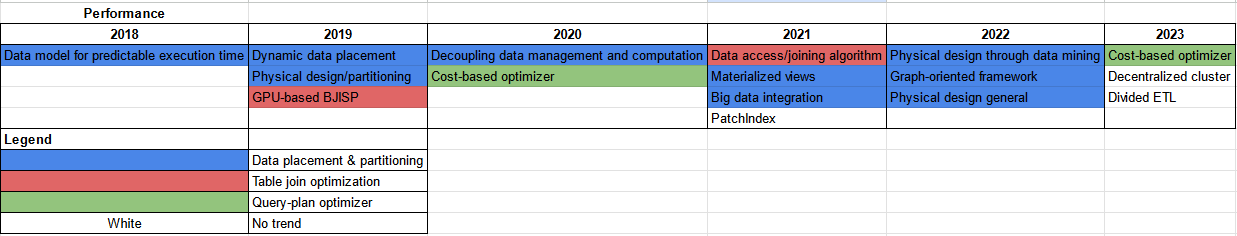
\includegraphics[scale=0.5]{Images/performance.png}
\caption{Categorizations of trends for performance}
\label{fig:performance}
\end{figure*}

\subsubsection{Schema design}
\label{results:trends:schema}
The biggest trend found regarding schema design is schema detection, generation, and evolution. Within this trend, most research was focused on automatic schema design and automatic schema evolution. The first paper on this topic was published in 2018 \cite{Taktak2018401}. 2018 also saw the start of two other trends, the first regarding temporal Data Warehouses (DWs)\cite{Gosain2018357}. A temporal DW is used to handle time-varying data in dimensions. The second trend is regarding the data cube \cite{Bantug2018}. A Data Cube design method allows for easier decision-making.

In 2019 research on schema detection and evolution continued with one more paper on schema detection from document-oriented data \cite{Bouaziz2019221}. In the same year, research on temporal DWs continued with one paper \cite{AinElHayat2019314}. Meanwhile, Data Cube's popularity rose with two more papers \cite{Djiroun2019783, Brahmi2019153}. Furthermore, two more trends were found in 2019. The first trend is the Data Vault design \cite{Kuznetcov2019}. The Data Vault method is most popular for allowing rebuilding the DW structure if the business model changes as well as dynamically expanding the DW model. The second trend is ontology-based schema design, which was also found in the section on data types, see section \ref{results:trends:types}. In 2019 four studies on ontology-based schema design were published \cite{Zekri2019273, Zekri2019285, Zekri20191190, Elamin2019}. \\

The introduction of the ontology-based schema design was immediately used to combine automatic schema design with ontologies in 2020, combining the first trend with this recently started ontology trend with a paper on automatic schema design from an ontology \cite{Hajji2020613}. Other works on schema detection and evolution were also published in 2020, with again the rise of applications in the domain of big data \cite{Nogueira202085}. Related to this topic a way to generate DW schemas from OLAP queries \cite{Huo2020337}. But also a new schema design method based on what was learned in previous work using business intelligence problem-solving thinking and a descriptive language model which allows for clearer communication surrounding a DW schema \cite{Takács20201}. The Data Vault methodology saw a continuation with one more paper combining the Data Vault design with a Metadata Vault Repository \cite{Jaksic2020813}. \\

2021 again saw more focus on applications of previous research on the domain of big data, in this case regarding semi-automatic schema generation for Big Data Warehouses \cite{Sautot202128}. Furthermore, two studies on automated schema construction using semantic data were published, one using a natural language processing framework \cite{Sanprasit2021518} and the other study, which similarly studied automated schema construction, but now looks more closely to semi-structured data \cite{Sanprasit2021}. Both these studies continue this mixed trend of ontology-based design with schema generation. In 2021 the Data Vault model continued to be studied, with a book chapter on the concept of the Data Vault model \cite{Gluchowski2021277} and a comparison between a Data Vault model and a snowflake model \cite{Grigoriev2021147}. This development shows that the Data Vault model is being taken seriously by researchers as a contender for a DW model. \\

In 2022 only the trend regarding schema generation continued with two papers on automatic schema generation, one using BI requirements and natural language processing \cite{Pizarro202213}, the other using machine learning to find the relevant analytical measures that are important for schema design \cite{Yang2022173}. The trend on temporal DWs also continued with one paper proposing a temporal data warehouse to solve the slowly changing dimension problem \cite{Phungtua-Eng2022214}. 2023 showed progress in the area of the Data Cube with one paper proposing a new Hyper Lattice structure \cite{Phogat2023697} and one more paper combining the data cube and a graph-based model with a temporal DW to create a temporal graph cube model \cite{Wang20231315}. \\

Again several papers did not belong to a specific trend. First, in 2018, a study proposed a DW design methodology that involves the end users more in the design process \cite{Sakka2018286}. Also in 2018, a study was published proposing a new schema for balanced performance and security in a cloud-based DW \cite{Karkouda20186}. In 2019 one study not belonging to a trend was published on a data store with a dynamic structure \cite{Artamonov2019794}. This study does relate somewhat to the evolving data and shift to NoSQL mentioned in previous sections but does not belong to any of the identified categories in this section. In 2020, one study presented a comparison of different schema designs in terms of performance \cite{Rocha202085}. Since the paper's main topic was schema design it was placed in this category but it does relate to performance trends a bit as well which were discussed in section \ref{results:trends:performance}. \\

The biggest trend regarding schema design was the rise in automatic schema detection, generation, and evolution. Furthermore, this category showed many overlapping trends with the rise of ontology-based design, which was also seen in other sections, and the mix of the data cube with a temporal DW and a graph-based model. This last combination also relates to section \ref{results:trends:types} where graph-based solutions were also used to handle NoSQL data which in turn relates to the rise of Data Lakes and Lakehouses discussed in section \ref{results:trends:architecture}. See figure \ref{fig:schema} for a graphical overview. \\

\begin{figure*}
\centering
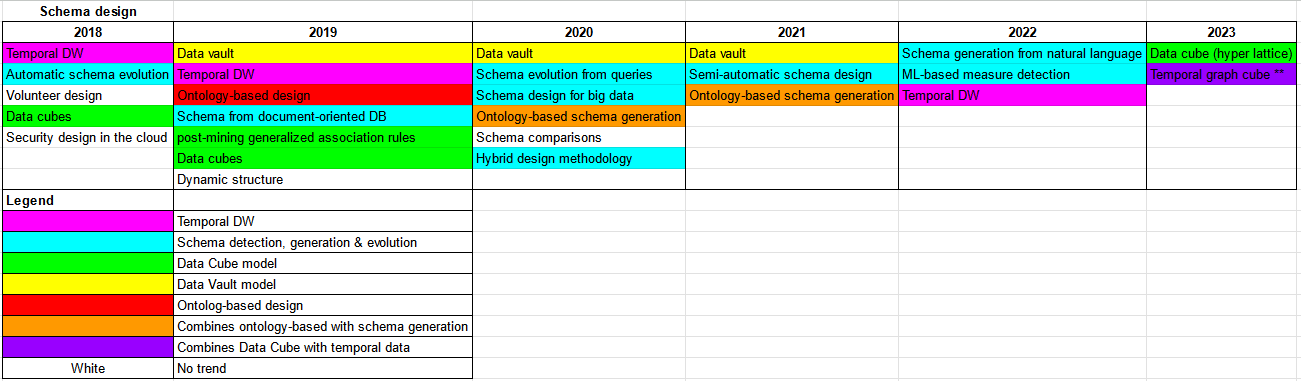
\includegraphics[scale=0.5]{Images/schema design.png}
\caption{Categorizations of trends for schema design}
\label{fig:schema}
\end{figure*}

\section{Future research \& approach}
\label{approach}
The information that is gathered with this review is a perfect stepping stone for future research. With the tooling, trends, and approaches that were found in this review, a framework can be created that can be used to determine which tools are most suitable for the data warehousing needs of a business or person. Before this framework can begin taking shape, the gathered information needs to be structured. The different tools should be analyzed in more depth to determine their technological and business strengths such that this can be matched with the needs of a user and the approach they want to take. Furthermore, the tools should be tested to see if they can handle certain trends that have emerged in the design and development of DWs to ensure the tools serve as a future-proof solution. For creating the framework it must also be determined how to shape the framework. For example, the framework can be a series of questions that narrow down the tools, but can also be a clear overview of the categorization from which users can see which tool would fit their needs. After this is determined the actual framework can be created. \\

The framework should then also be tested. This will be done in the form of a case study for Topicus .Finance. The focus within Topicus .Finance lies on three main sectors, namely pension and wealth \cite{pension},  mortgages \cite{mortgages}, and lending \cite{businesslending}. Within each of these sectors, Topicus .Finance has multiple software applications for individuals or companies. During the case study, one of these software applications for the lending side will be used as the basis for a case study. The application is called Fyndoo \cite{fyndoo}, and is used by almost all major banks and many smaller banks and other financial institutions that offer lending services in the Netherlands. Fyndoo is a software application that streamlines the lending application process for both the financial institution and the applicant. Within Fyndoo Topicus .Finance wants to give their clients more insight into their processes as well as help them with the reporting they need to do to "De Nederlandsche Bank" (DNB), which in turn reports to the European Central Bank (ECB). These problems can both be solved with the use of a data warehouse which means this case is very suitable as a test for the framework. \\

After the framework is applied on Topicus .Finance's situation, a data warehouse will be designed and built with the tools that were suggested by the framework. This implementation will also require insight into the client of Topicus .Finance. Therefore, interviews will be conducted with these clients to gather information on the processes these clients wish to monitor and which reporting needs they still have. From these interviews, the Key Performance Indicators (KPIs) can be found which will help in the design of the data warehouse. Lastly, the implemented solution has to be evaluated. First with the clients to see if the new features of Fyndoo are helpful. Second the framework has to be evaluated with Topicus .Finance to see if the implemented solution is also a good fit for them. The framework should also be further evaluated with different parties in terms of usefulness and clarity. This can be done by sending out a survey to anybody with a technological background in data science, data warehousing, or who is otherwise proficient with data. With these evaluations, it should be possible to see if the framework is useful or not. \\

% \begin{figure*}[ht]
%     \begin{center}
%     \begin{ganttchart}[y unit title=0.4cm,
%     y unit chart=0.5cm,
%     vgrid,hgrid, 
%     vrule/.style={very thick, green},
%     vrule label font=\bfseries,
%     title label anchor/.style={below=-1.6ex},
%     title left shift=.05,
%     title right shift=-.05,
%     title height=1,
%     progress label text={},
%     bar/.append style={rounded corners=3pt},
%     bar height=0.7,
%     group right shift=0,
%     group top shift=.6,
%     group height=.3]{1}{21}
%     %labels
%     \gantttitle{Week}{21}\\
%     \gantttitlelist{1,...,21}{1} \\\\
%     %tasks
%     \ganttbar[bar/.append style={fill=purple}]{Prepare and plan interviews}{1}{2} \\
%     \ganttbar[bar/.append style={fill=violet}]{Conduct and analyse interviews}{3}{10} \\
%     \ganttbar[bar/.append style={fill=orange}]{Match tools with practice}{2}{7}\\
%     \ganttbar[bar/.append style={fill=magenta}]{Categorize tools}{2}{7}\\
%     \ganttbar[bar/.append style={fill=cyan}]{Create framework}{6}{9}\\
%     \ganttbar[bar/.append style={fill=yellow}]{Apply framework to Topicus}{10}{11} \\ 
%     \ganttbar[bar/.append style={fill=blue}]{Design and implement data warehouse}{12}{17}\\ 
%     \ganttbar[bar/.append style={fill=red}]{Evaluate solution \& framework}{18}{18} \\
%     \ganttbar[bar/.append style={fill=lime}]{Extension}{19}{20} \\
%     \ganttbar[bar/.append style={fill=pink}]{Presentation}{20}{21} \\
%     \ganttbar[bar/.append style={fill=teal}]{Writing}{2}{21} \\
%     \ganttvrule{Green light}{17}
%     \end{ganttchart}
%     \caption{Gantt chart of preliminary planning final project}
%     \label{gantt_chart}
%     \end{center}
% \end{figure*}

% \section{Planning}
% \label{planning}
% Figure \ref{gantt_chart} shows the preliminary planning for this future research. The first eleven weeks will be used for completing all analysis components of this research. In these eleven weeks, the interviews for the case study will already be completed and analyzed. Since the interviews will be dependent on the availability of the clients of Topicus .Finance it is preferable to have these planned early to stay on schedule. Parallel to these interviews, the tooling and approaches must be analyzed in more depth as discussed in the approach in section \ref{approach}. Furthermore, decisions have to be made regarding the tooling to be used for the implementation of the data warehouse. Moreover, the different nature of each of these tasks gives a balance in the type of work that is required to complete them. This can help with motivation and focus as performing the same task for a long time can be very exhausting and can lead to a lack of focus. The next six weeks will be used to design and implement the data warehouse. The final four weeks are used to receive feedback on the developed solution and the framework, finish writing the report, and prepare for the presentation. These weeks also allow for a little extension if parts carry on for longer than expected.

\section{Conclusion \& limitations}
In conclusion, this paper first discussed the available open-source DW tools that are currently available. By using a combination of literature and search engine results a list of 31 tools was found. After applying inclusion and exclusion criteria, 25 tools remained. The tools vary from full-fledged user interface with drag-and-drop capabilities for users with limited programming experience to simple Python libraries that help group tasks together into pipelines. \\

Next, the current trends and approaches in the research, design, development, implementation, or improvement of a data warehouse were investigated through a systematic literature review. Previous studies had done similar work up until 2018, this paper therefore focussed on everything from 2018 until February 2024. The final result consisted of 126 papers. For the DW architecture, the data lake and the lakehouse are becoming more popular. The concept of data lakes has been extensively researched over the past years to tackle any challenges that were faced while using a data lake. For the design approach, the work of Kimball et al. \cite{kimball2011data} is still popular. Other approaches were mentioned too, but not as often as the nine steps outlined by Kimball. For the data model design, most research was focused on automatic schema creation and automatic schema updating. Another big trend was ontology-based schema design. This ontology-based approach also emerged in research that aimed to deal with new types of data. Especially linked open data and IoT data are popular topics. Furthermore, trajectory data of moving objects was also mentioned several times. These types of data also resulted in more work on NoSQL databases as these are very suitable to deal with a plethora of data types. Research on ETL is mostly focussed on near real-time ETL as the demand for fast data analytics is growing. Another big trend in ETL research is data quality and enrichment. The importance of ensuring clean data was already clear, the current research mostly suggests new, more efficient ways of cleaning and enriching. Lastly, studies on performance improvement showed two main trends. The first is the physical design of the system in combination with data placement. The second trend is focused on query optimization and efficiency. \\

The limitations of this study lie in the collection of relevant literature. First of all, as mentioned before and as the results show, the literature on open-source tooling was very limited. Adding search engine results made sure a complete overview of tools could be made but the threat in this approach is that the results are not proved scientifically. The impact of this threat however is very limited, as the goal of RQ1 was to find a complete overview of software that is used on a daily basis in both professional and smaller-scaled settings. \\

Second of all, there is a threat of validity to the collection of relevant literature for RQ2. The threat in this part is twofold. First, data warehousing is a very hot topic for research which means that a search query like the one used in this study retrieved almost 750 papers. While the use of inclusion and exclusion criteria to narrow these papers down worked well, there is a possibility that papers were excluded even though they did contain relevant information. This threat was mitigated as much as possible by dividing the work into smaller portions to ensure that there was no lack of focus during the review process. Second, the result is currently limited to only Scopus. While it was indicated as the most comprehensive and user-friendly literature database \cite{harzing2016google, mongeon2016journal} and in total 126 papers were covered in this study, it is possible that other literary databases included papers that are also relevant to this topic. Nevertheless, the number of papers is seen as enough to cover the trends that have emerged since 2017.

% Entries for the entire Anthology, followed by custom entries
\printbibliography
\onecolumn
\appendix

\section{Overview of tools}
\label{appendix:tools}
\begin{table}[H]
\centering
    \begin{tabular}[c]{|p{2cm}|p{4cm}|p{4cm}|p{1.5cm}|p{4cm}|}
    \hline
    \textbf{Name} & \textbf{UI/Code} & \textbf{Git rating/community size} & \textbf{Paid option} & \textbf{Notable features} \\ \hline
    Airbyte & UI, Terraform,and API & 13.2k stars, 863 contributors & Yes & DBT for transformations \\ \hline
    Apache Airflow & UI and Python & 33.5k stars, 2804 contributors & No &  \\ \hline
    Apache Beam & Python, Java, GO, typescript, Scala, SQL, YAML & 7.4k stars, 1170 contributors & No & Multi-language pipelines \\ \hline
    Apache Camel & Java & 5.2k stars, 1029 contributors & No & Integration tool with ETL \\ \hline
    Apache Druid & Web UI with SQL queries & 13.1k stars, 591 contributors & No &  \\ \hline
    Apache Hadoop & MapReduce & 14.2k stars, 573 contributors & No & Cluster computation \\ \hline
    Apache Hive & CLI & 5.3k stars, 372 contributors & No &  \\ \hline
    Apache Hop & GUI + web, CLI tools & 813 stars, 70 contributors & No & Based on Pentaho \\ \hline
    Apache Kafka & Java and Scala & 26.9k stars, 1105 contributors & No & Real-time streaming \\ \hline
    Apache NiFi & Web UI, & 4.2k stars, 459 contributors & No &  \\ \hline
    Apache SeaTunnel & CLI & 7k stars, 252 contributors & No &  \\ \hline
    Apache Spark & Python, Java, R, Scala, SQL & 37.9k stars, 2042 contributors & No & Big data analysis \\ \hline
    CloudQuery & CLI & 5.4k stars, 142 contributors & Yes & Transformation with DBT \\ \hline
    Dagster & Python and Web UI & 9.7k stars, 380 contributors & Only paid & Integrates with DBT and Airbyte \\ \hline
    DBT & CLI, SQL & 8.5k stars, 290 contributors & Yes & Integrates well with other tools \\ \hline
    Kestra & Localhost GUI with IDE & 5.4k stars, 194 contributors & Yes & Integrates with Airbyte and DBT \\ \hline
    Knime & GUI & 144 stars, 17 contributors on GitHub & Yes & Has own community platform \\ \hline
    Mage & GUI or own IDE, Python, R and SQL & 6.6k stars, 92 contributors & No &  \\ \hline
    Meltano & CLI & 1.5k stars, 120 contributors & No & Transformation with DBT \\ \hline
    Pentaho Community edition & Low-code GUI & 7.2k stars, 221 contributors & No &  \\ \hline
    Prefect & Python + monitoring UI & 14.1k stars, 227 contributors & Yes &  \\ \hline
    PipelineWise & CLI & 597 stars, 45 contributors & No & Requires Singer \\ \hline
    Python libraries\text{*} & Code & NA & No & Scheduling with cron \\ \hline
    R\_etl & R & NA & No & Dedicated R package \\ \hline
    Singer & CLI & $\sim$1.5k stars, $\sim$30 contributors & No & PipelineWise scheduling and monitoring \\ \hline
    \end{tabular}
    \caption{\text{*}The Python libraries include: Ethereum-etl, Luigi, Petl, Pygrametl}
\end{table}

The programming language is mentioned if the tool uses code as its main way of building ETL pipelines. If the application is more low/no code, this is indicated in the UI used. Sometimes both options are possible while other times a UI is only for monitoring the pipelines, not for building.

\end{document}
